\chapter{Introduction}
\begin{figure}[h]
\centering
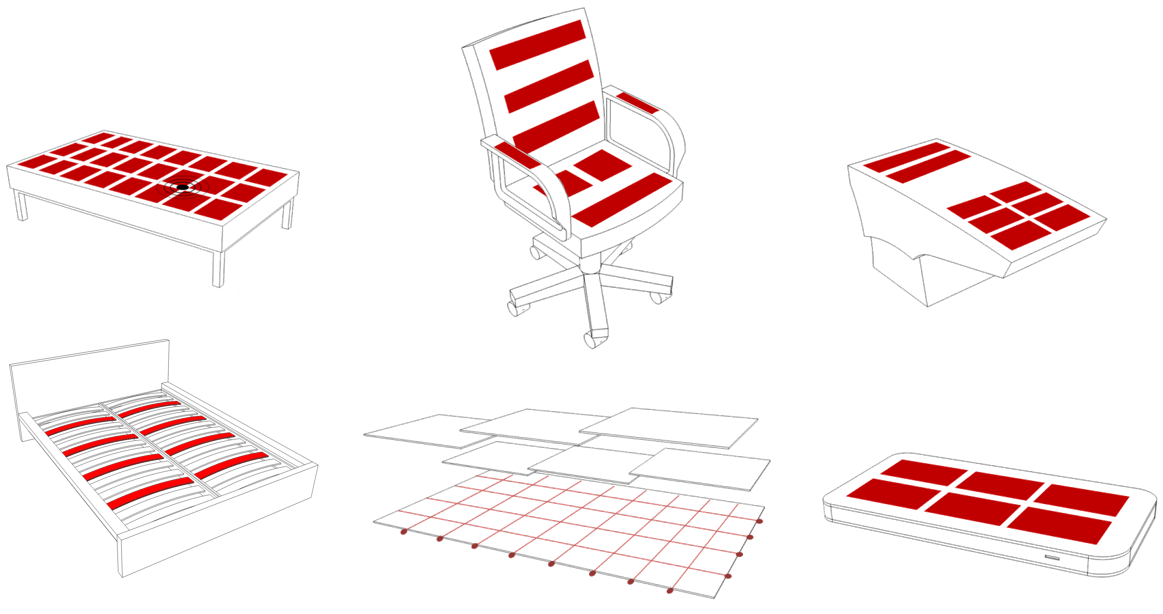
\includegraphics[width=0.9\textwidth]{images/all_protos}
\caption{Sketch of electrode placement of all capacitive sensing prototypes created in the scope of this work}
\label{fig:all_protos}
\end{figure}
Smart environments are comprised of numerous sensing and computing devices that are supporting a number of users in this environment on performing their tasks. Driven by advances in computing power, miniaturization of sensors and processing methods, novel devices including a plethora of functionality have been introduced into our everyday lives.  In science the field has been thriving in the last decades, combining knowledge from disciplines including computer science, engineering, but also product design, in order to create systems that are integrated into the environment, have a high usability and provide information and services to the actors in smart environments. Perhaps the most cited example of this trend is the rise of the smartphone, from professional business tool to a consumer device being sold hundreds of millions times a year. Using integrated sensors and communication facilities it is possible to provide services aware of location, schedule, contacts, or preferences, that realize navigation, event planning, augmented reality, or entertainment. A different example are increasingly networked homes that are aware of energy usage, lighting levels, temperature and the status of critical devices and can be controlled by the user from a single place or autonomously using a set of specified rules. 

A common aspect of all smart environments and smart devices is sensing. This includes environmental parameters but also system state and most importantly the activities of the different users. There are numerous categories of sensing devices that can realize different aspects of this sensing, ranging from cameras or accelerometers to GPS and acoustic sensors. Capacitive sensors are a category of sensors that use electric fields to sense the presence and certain properties of the human body. The most common variety is sensing the presence of fingers on touch screens, already present in billions of devices. However, there is another variety, the capacitive proximity sensor that is able to detect the presence of human body parts over a distance, providing interesting applications in smart environments, by unobtrusively integrating the sensors into different materials, environments and appliances. When designing an application of smart environments choosing the right sensors is one of the most relevant decisions that has to be taken early in the process. Even though there are numerous prototypes available, so far this process has been mostly supported by looking at previous activities. 

In this work I present a benchmarking model that can support this decision process in the domain of smart environments, in order to determine relevant application areas for capacitive proximity sensors. There are numerous challenges associated to each area, regarding the details of the application. I will present a collection of existing and novel methods that support processing data generated by capacitive proximity sensors. Several prototypes created using those methods have been implemented and evaluated for performance and usability. Figure \ref{fig:all_protos} shows sketches of the different prototypes and the placement of the electrodes attached to the capacitive proximity sensors. Based on this evaluation and the knowledge generated in the design process I am able to discuss the benefits and limitations of the technology, classify it with regards to competing technology, in order to present a set of guidelines that can aid parties interested in designing smart environment applications using capacitive proximity sensors.
 
\section{Motivation}
In the last decade the way we interact with computing machines has changed in a profound fashion. Today more than one billion people operate a smartphone, enabling ubiquitous access to communication tools, processing power and information. The vision of ubiquitous computing as proposed by Mark Weiser in the early 90s is inching closer to reality \cite{Weiser1991}. The required technologies of \begin{quote}
"cheap, low-power computers that include equally convenient displays, a network that ties them all together, and software systems implementing ubiquitous applications" 
\end{quote}
are now existing in the form of smartphones and tablets that are connected to the internet, using high-speed connections such as LTE and web-based services such as Google Now, that combine numerous data sources to provide personalized services.

While the vision and underlying ideas remain similar other names have been used in research, including Pervasive Computing and Ambient Intelligence. The concept has been expanded to not only consider devices that can be directly manipulated, but include determining the situation and reacting based on it. This context-aware computing proposes 
\begin{quote}
"systems that examine and react to an individual's changing context. Such systems can promote and mediate people's interactions with devices, computers, and other people" \cite{schilit1994context} 
\end{quote}
Different forms of context can be distinguished, ranging from location and the actual system state, to different activities or even the current mood of the user. In order to acquire this context, the input-and-output based systems originally proposed by Weiser, are augmented by an ensemble of devices that are very small (dust), coordinate in massive numbers (clay) or are flexible, unobtrusive extensions to everyday objects (fabric) \cite{poslad2011ubiquitous}. This devices can be invisibly integrated into our everyday environment and provide sensing capabilities that can be used by sufficiently smart systems. Examples of these devices are microelectromechanical systems (MEMS) or bendable technology, such as OLED screens. The number of computation and sensing devices that we carry with us is growing continuously, yet we want the technology to further disappear, allowing us to focus on the application instead of the underlying technology. 

The famous science fiction author Arthur C. Clarke proposed three laws of prediction, the third of which is 
\begin{quote}
"Any sufficiently advanced technology is indistinguishable from magic." \cite{clarke1962hazards} 
\end{quote}
Capacitive proximity sensing allows us to measure the influence of the human body (or conductive objects in general) on an electric field. While this technology is not magic per se, a peculiarity of electricity is that humans, as opposed to some animals, have no specific sensing organs for this property. Thus we remain unaware of their presence, unless the field strength is very high. Consequently, when interacting with capacitive sensors there is no awareness of what they are sensing unless it is specifically exposed to another sense of the user, such as haptic feedback on touch screens or visual feedback on touch less systems. Touch screens are the most ubiquitous application of capacitive technology, being applied in all modern smartphones and tablets, thus being used by a large number of the world's population every day. However, they are typically tuned to only register touches, while other varieties are also able to detect objects over a distance. This enables numerous other applications for this technology, ranging from industrial fluid level and material detection, to presence detection in cars. A particularly interesting domain for this sensing technology are smart environments that provide services based on unobtrusively acquired information about persons currently acting in this environment. A popular capacitive proximity sensors have been primarily used for human-computer interaction (HCI) applications, including a mouse tracking the distance of the heel of the hand or a monitor that is able to track gestures performed in front of it. Another area are smart appliances, such as an object detecting car seat or localization systems. There are numerous sensing technologies that provide similar detection capabilities. Looking at the recognition of simple activities, such as standing, walking and lying, cameras and accelerometers can lead to the same result. Thus, it is often difficult to decide what the specific sensor technology to use in a specific system. Commonly one refers to previous work and best practice, building on previously generated knowledge. However, so far there is no formal model that would allow to quickly evaluate different sensor technologies in different applications. Taking into account a specific set of features required for a specific application domain this could be an important decision support tool in the early stages of system development. As it was stated by Cook and Das \cite{cook2007smart}:
\begin{quote}
"Finally, a useful goal for the smart environment research community is to define evaluation mechanisms. While performance measures can be defined for each technology within the architecture hierarchy [...], performance measures for entire smart environments still need to be established. This can form the basis of comparative assessments and identify areas that need further investigation."
\end{quote}
Such a tool can also be used to identify specific applications for a single sensor technology, such as verifying current and developing new use cases for capacitive proximity sensors or providing a classification of the technology with regards to competing sensor systems. However, identifying a suitable sensor is just the first step in designing a smart environment prototype or product. After this decision a designer has to determine specific challenges of the domain, select suitable methods for applying the technology and processing the data and create a working system. In this design step it is helpful to have a set of methods, examples and guidelines, leading to a more rapid prototyping for researchers and shorter time-to-market for product developers. These guidelines should be the result of literature review and validating prototypes for performance and usability. 

\section{Research Challenges}
In the past there have been numerous influential works that gave an overview of technologies and applications in smart environments. Cook et al. identified common technologies, frameworks and applications in this domain and give an overview of ongoing research \cite{cook2007smart}. Poslad specified a more detailed taxonomy of device classes, provides concepts for interaction between humans and environments and gives an overview of intelligent systems \cite{poslad2011ubiquitous}. A different category of previous work details the different sensing technologies that are supporting various different applications and give an overview of limitations and benefits. However, so far there has been no work that provides a benchmark that maps different sensor characteristics to applications in smart environments. An intermediate step between evaluating entire environments and low-level technologies is an application-specific benchmarking of systems. Benchmarking as a method allows us to quantify the performance of a specific process or item and allows a comparison to competing processes or items. It is common to benchmark different technologies according to their features. My proposal is to extend technology-driven benchmarks by adding an application-specific feature weighting. This approach allows to map the same set of features to different applications that have similar requirements that are catered to by divergent technologies. It will be verified by benchmarking typical applications with regards to several example applications in the domain of smart environments.

The selection of application scenarios for capacitive proximity sensors is mostly based on previous works, most notably by research groups from MIT \cite{Paradiso2002}, Disney research \cite{Sato2012} or the Munich University of Technology \cite{Wimmer2006}. They are extending on the methods or modify existing use cases to another domain. Using the developed benchmarking method it is possible to verify the existing application areas or even determine new ones. It also allows to specify if other sensing technologies might be more suitable for a specific application. This allows to identify four relevant application domains that can be realized with capacitive proximity sensors. 

Following the design process a next step is specifying the particular challenges for the given application, selecting suitable processing methods, in order to create and evaluate a system. Looking at the related works several areas are identified that can be improved using novel or adapted methods. E.g. previous systems often rely on uniform sensor arrays \cite{Smith1996a} or require a large number of sensors \cite{rekimoto2002smartskin}. Improvements are proposed for object tracking using a low sensor count, unobtrusive localization in large areas, model-driven approaches for object fitting and heterogeneous sensor systems , fusing different geometries or sensor categories. The presented methods are realized in different prototypes that are evaluated for usability and performance.
Using the knowledge generated from determining applications, finding specific challenges and creating different prototypes I am able to classify capacitive proximity sensors with regards to other sensing technologies in the domain of smart environments. It is possible to identify specific benefits and limitations and compare features between technologies. This culminates in creating a set of guidelines for parties that are interested in developing smart environment systems based on capacitive proximity sensors.

%In addition to the work on capacitive proximity sensors I have also worked on various other aspects regarding interaction in smart environments and indoor localization.  Pointing at devices in order to control them is an intuitive way of interaction, often unconsciously performed when switching TV stations with an infrared remote, even though it is usually not required. However, only a limited number of devices have the required facilities for this kind of interaction since it does require attaching transceivers and often results in the necessity to use multiple remote controls. I propose a system giving a user the ability to intuitively control arbitrary devices in smart environments by identifying the appliance an interaction device is pointed at and providing means to manipulate these. The system is based on identifying the position and orientation of said interaction device, registering these values to a virtual representation of the physical environment, which is used to identify the selected appliance. 

%Indoor localization is a base technology within smart environments, enabling a multitude of applications including augmented reality, navigation in large indoor areas, or sports \cite{thomas2000arquake, ingram2004ultrawideband, leser2011local}. Some particular challenges in assisted living applications include low budgets, easy installation, privacy preservation and interoperability with other systems in the environment \cite{chessa_eval}. Camera-based systems are very popular in this domain, yet particularly in private settings struggle with user acceptance. A potential solution are smart camera systems that process and abstract the images before they are sent to the network, however they require efficient and robust tracking algorithms for implementation on embedded systems. 
 
\section{Contributions}
In the following I will list briefly and concisely what are the specific contributions provided by this work on a methodological and practical level. They are distinguished into three different groups, the benchmarking model, the validation of capacitive proximity sensors and additional smart environment research topics.

I will introduce a generic and formal benchmarking model for sensor systems in smart environments. This includes the identification of relevant sensor features that should be included in the scoring process, leading to a feature matrix that links features to ratings. Based on an importance-based weighting process a benchmark score calculation is presented, including methods to normalize the score based on average feature scores. This benchmarking model is used to identify different use cases for capacitive proximity sensors in the domain of smart environments.

In order to validate the sensor technology different challenges are determined for each use case, allowing to identify processing methods that can be beneficial. Processing methods in five different groups are presented. Two methods for sparse sensor configurations that enable tracking hand gestures in three dimensions and localization and fall detection in large areas. Several model-driven fitting methods applying machine learning on single- and multi-body models. Methods for processing in heterogeneous sensor systems comprised of non-uniform array configurations, parallel processing of single data streams or fusion of different sensor systems. Considerations regarding image-based processing for loading mode sensors in uniform array configurations. Several methods to process physiological signals using different sensing modes in frequency- and time-domain. 

Six different prototypes are detailed and evaluated. The MagicBox prototype, enabling expressive single-hand gestural interaction with sparse sensor distribution and machine learning gesture classification. The CapFloor system, using a novel layout for floor-based capacitive indoor localization systems, enabling unobtrusive application, easy maintenance and additional services such as fall detection. The SmartBed prototype using a model-based approach for fitting one or two persons, concurrently detecting sleep phases and breathing rate for occupants. The Capacitive Chair smart furniture that allows to detect presence, identify users, track different postures, measure breathing rate and enables novel applications for smart offices. The Active Armrest using a heterogeneous sensor layout to enable different forms of interaction in automotive environments. The CapTap prototype combining capacitive sensors and microphones in a table-based interaction device, enabling multi-hand gesture recognition in three dimensions using a multi-level interaction pattern. Three other prototypes, CapDisp, HoneyFish and GestDisp, that were created in collaborative efforts are described briefly.

The last group is comprised of other topics in smart environments focus on presenting a marker-free interaction paradigm for pointing-interaction with arbitrary devices in smart environments, showing multi-modal use cases and different bounding volume modification techniques in the virtual realm. The second system is AmbiTrack - a camera-based indoor localization system for smart environments, initially designed to calibrate and evaluate capacitive systems.


%\item Image-based processing methods for loading mode sensors
%\item Processing of physiological signals in frequency- and time domain
%\begin{itemize}
%\item Benchmarking model for sensors in smart environments
%\begin{itemize}
%\item Identification of application domains in smart environments
%\item Application-centric benchmarking model for mapping a single set of sensor features to different smart environment applications
%\item Identification of applications suitable for capacitive proximity sensors based on the developed benchmarking model
%\end{itemize}
%\item Validation of capacitive proximity sensors in smart environments
%\begin{itemize}
%\item Specifying challenges in the presented application domains
%\item Improved processing methods related to these challenges
%\begin{itemize}
%\item Processing methods for sparsely distributed sensor arrays including 3D hand tracking and large-area localization
%\item Model-driven fitting methods using machine-learning methods on single-, and multi-body models
%\item Heterogeneous sensor systems comprised of non-uniform array configurations, parallel processing of single data streams and fusion of different sensor systems
%\item Image-based processing methods for loading mode sensors
%\item Processing of physiological signals in frequency- and time domain
%\end{itemize}
%\item Application prototypes
%\begin{itemize}
%\item MagicBox prototype enabling expressive single-hand gestural interaction with sparse sensor distribution and machine learning gesture classification
%\item CapFloor prototype using a novel layout for floor-based capacitive indoor localization systems, enabling unobtrusive application, easy maintenance and additional services such as fall detection
%\item SmartBed prototype using a model-based approach for fitting one or two persons, concurrently detecting sleep phases and breathing rate for occupants
%\item Capacitive Chair prototype that uses allows to detect presence, identify users, track different postures, measure breathing rate and enables novel applications for smart offices
%\item Active Armrest prototype uses a heterogeneous sensor layout to enable different forms of interaction in automotive environments
%\item CapTap prototype combining capacitive sensors and microphones in a table-based interaction device, enabling multi-hand interaction in three dimensions using a multi-level interaction pattern
%\item Short description of CapDisp, Honeyfish, GestDisp
%\end{itemize}
%\item Discussion of limitations and benefits of capacitive proximity sensors in smart environments and comparison to other sensing technologies
%\end{itemize}
%\item Interaction and localization in smart environments
%\begin{itemize}
%\item Marker-free interaction with arbitrary devices in smart environments
%\item Presentation of AmbiTrack - a camera-based indoor localization system for smart environments
%\end{itemize}
%\end{itemize}

\section{Structure of this work}
After having identified the research challenges and introduced the topic the related works are specified in Section \ref{ch:related_work} - \emph{\nameref{ch:related_work}} - in four categories. The first section gives a background on electric field sensing, including relevant historical work and the physical properties. Additional different sensing categories are outlined, before different electrode considerations and data processing methods are introduced. The second category of related works discusses different applications of capacitive proximity sensors that were created in the last decades, ranging from MIT research in the early 90s, to novel touch classifiers based on different sensing methods. The third category introduces different competing technologies that will be used in the later benchmarking. Finally we give an overview of existing work collecting and grouping applications in smart environments. This will allow us to identify candidate scenarios for capacitive proximity sensors.

Section \ref{ch:benchmark} - \emph{\nameref{ch:benchmark}} - is concerned with the first main contribution of this work, the introduction of an application-specific benchmarking model for sensors in smart environments. In the first part of this section the sensor features relevant for application in smart environments are discussed. Suitable features are discussed in three different categories, discussing the rationale for inclusion or omission in the model. The next part describes the benchmarking model. The application-based feature weighting is introduced, leading to the derivation of the model itself, including the required calculation of an overall rating and a feature score normalization. After that we are using the model to score different examples and validate those using search results from scientific publication databases. Afterwards, the model is discussed and used to identify suitable applications for capacitive proximity sensors in smart environments.

Section \ref{ch:usecases} - \emph{\nameref{ch:usecases}} - describes the identified use cases for capacitive proximity sensors in smart environments. First, the use cases and associated challenges for design and processing are identified. Afterwards different processing methods for capacitive proximity sensors are presented that tackle the specific challenges. This includes methods for sparsely distributed sensor arrays, model-based data fitting, heterogeneous sensor systems, image-based processing and physiological signal processing. Six different prototypes that implement one or more of the processing methods are presented and evaluated - MagicBox, CapFloor, Capacitive Chair,  Active Armrest, SmartBed and CapTap. Each of the prototypes has been evaluated for performance and usability. Additionally, three other prototypes are discussed briefly.

The knowledge gathered in designing, building and testing the prototypes and using the benchmarking model leads to Section \ref{ch:eval} - \emph{\nameref{ch:eval}}, wherein the results are discussed and evaluated. This section has four parts. At first capacitive proximity sensors are compared to the other sensor classes introduced in the related works. Afterwards limitations and benefits of the technology are collected and linked to the sensor features and applications. The section concludes with a set of guidelines that may help interested parties in evaluating their application for usage with capacitive proximity sensors and give practical help when applying this technology.

%Section \ref{ch:pointing} - \emph{\nameref{ch:pointing}} - is introducing a system, enabling pointing interaction with arbitrary devices in smart environments without requiring markers. Using integrated and external sensors it is possible to detect the location and orientation of an interaction device and register it into the virtual domain, where appliances can be identified. This includes methods improving this interaction pattern, such as multi-modal adaptation and strategies for bounding volume modification of registered devices.

%Section \ref{ch:ambitrack} - \emph{\nameref{ch:ambitrack}} - is presenting a camera-based indoor localization system. While this section is not directly concerned with capacitive proximity sensors, indoor localization is an important technology for numerous smart environment applications. AmbiTrack has been created for participating in the EvAAL competition that evaluated different indoor localization systems for Ambient Assisted Living, ranking the systems based on numerous technical features, user experience and openness of implementation. The section will briefly introduce the requirements for indoor localization systems and present the prototype system and results of the EvAAL competition.

The document concludes in Section \ref{ch:conclusion} - \emph{\nameref{ch:conclusion}} - that briefly recapitulates the work and introduces potential future research stemming from this work.

There are four different appendices. Appendix A includes raw results and additional material of the evaluations performed with the different prototypes. Appendix B lists publications and talks. Appendix C lists Master and Bachelor Thesis that were supervised or co-supervised. Appendix D contains a short CV.